\begin{frame}{Métricas disponíveis no Bench4Q}
	Nesta seção é descrito de maneira detalhada a implementação realizada no \textit{benchmark} Bench4Q e a abordagem utilizada no processo. Descrevemos também as implementações das distribuições de carga de trabalho e as disponibilizamos sob uma licença de código aberto, com o intuito de que outros possam reutilizar a plataforma desenvolvida e estender o \textit{benchmark} segundo as suas necessidades para contribuir com outros tipos de modulação de cargas de trabalho num ambiente de experimentos controlado~\footnote{O código fonte está disponível em \href{URL}{http://gitlab.lasdpc.icmc.usp.br/edwin/bench4q}}.
	
	Dentro do processo de experimentos de sistemas de computação em nuvem onde é analisado o comportamento da resposta a uma perturbação no regime transiente, foram identificadas algumas faltas de funcionalidades fundamentais, principalmente na geração da carga de trabalho. Especificamente, o Bench4Q possui algumas limitações na sua versão original, principalmente pela definição do próprio projeto de \textit{software} para avaliação de desempenho no regime estacionário. Esta limitação foi uma barreira que dificultou a experimentação e analise nos trabalhos relacionados com o presente projeto de \cite{Edwin2015} e \cite{Lourenco2015}.
\end{frame}

\begin{frame}{Métricas disponíveis no Bench4Q}
	O Console do Bench4Q é o módulo que gerencia EBs para gerar uma série sequencial programada de requisições que são submetidas para o SUT. O tópico aqui é controlar a taxa em que os EBs geram as requisições, para que seja possível controlar diretamente e de forma programada a carga de trabalho. Nativamente o Bench4Q, coleta informações sobre a taxa requisições e o comportamento do SUT, e relata esses dados no final da experimento. A Figura \ref{fig:experimental-setup} ilustra de maneira geral o fluxo desse contexto.
	
	\begin{figure}[htb]
		\centering
		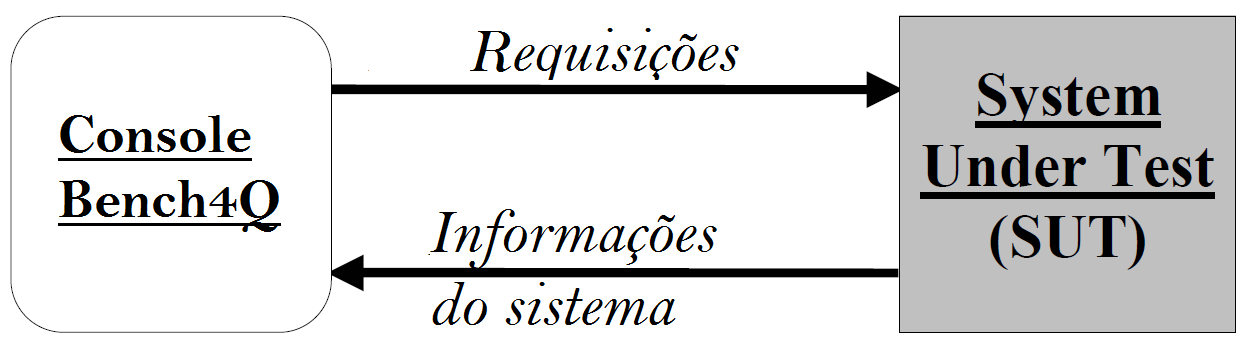
\includegraphics[scale=0.2]{../monograph/images/experimental-setup.png}	
		\label{fig:cps-resp60}
	\end{figure}
	
\end{frame}

	
\begin{frame}{Métricas disponíveis no Bench4Q}
	\begin{figure}[htb]
		\centering
		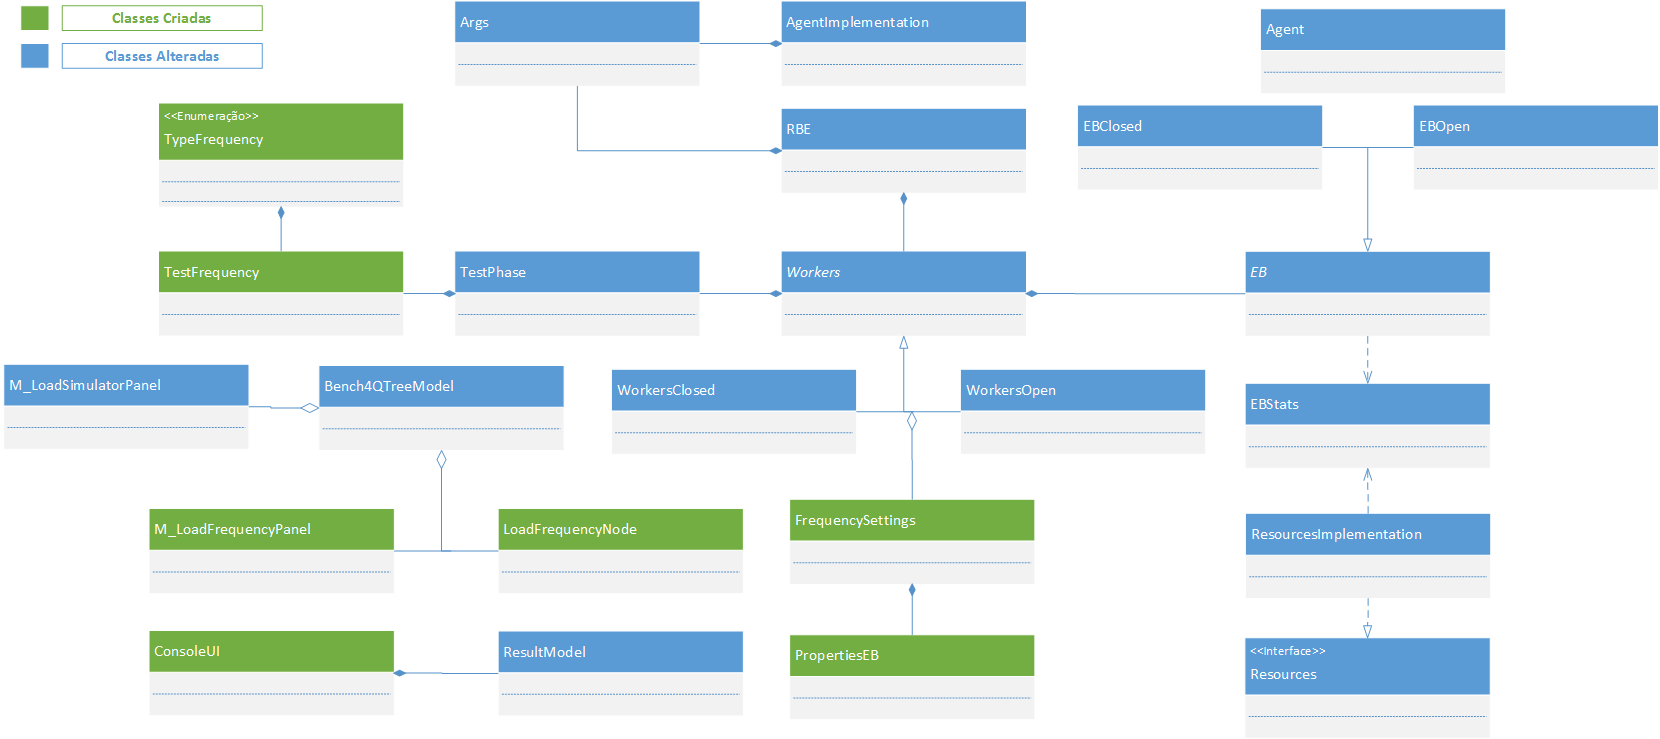
\includegraphics[scale=0.3]{../monograph/images/diagrama-classes-beanch4Q.png}	
	\end{figure}
\end{frame}

\begin{frame}{Teste de modulação}
	\begin{figure}[!htb]
		\centering
		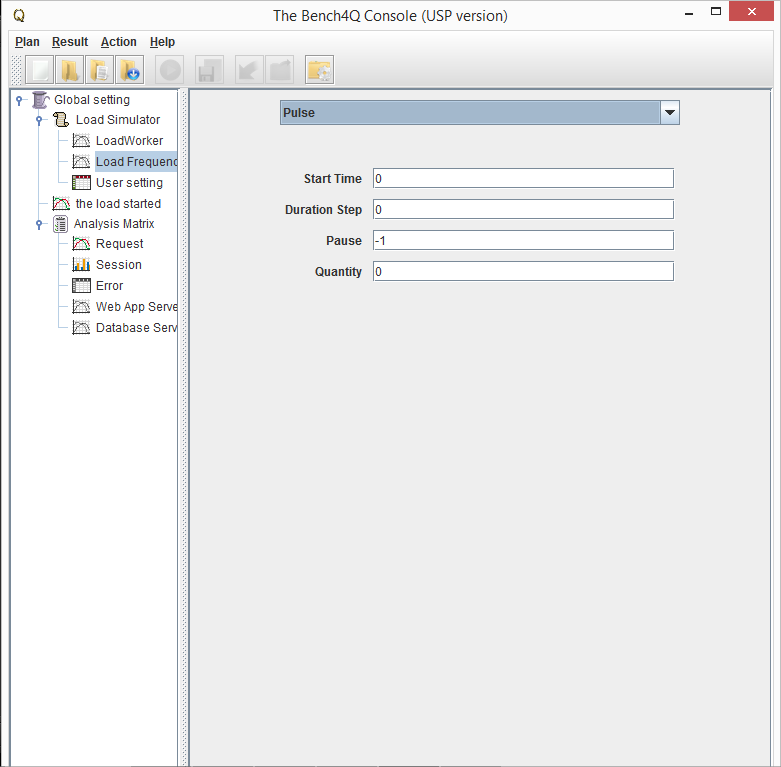
\includegraphics[scale=0.3]{../monograph/images/console-bench4Q-usp.png}
		\caption{Console de programação da carga de trabalho.}
		\label{fig:interface-criada-beanch4q}
	\end{figure}
\end{frame}

\begin{frame}{Teste de modulação}

\end{frame}

\begin{frame}{Teste de modulação}
	\begin{figure}[!htb]		
		\begin{subfigure}{\linewidth}
			\centering
			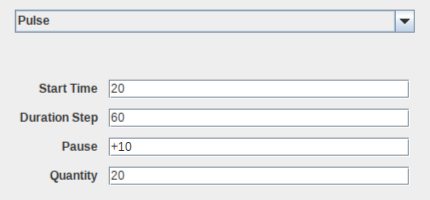
\includegraphics[scale=0.35]{../monograph/images/condiguracao-carga-modulada1.png}
			\label{fig:configuracao-carga-modulada-teste}
		\end{subfigure}\\[1ex]
		\begin{subfigure}{\linewidth}
			\centering
			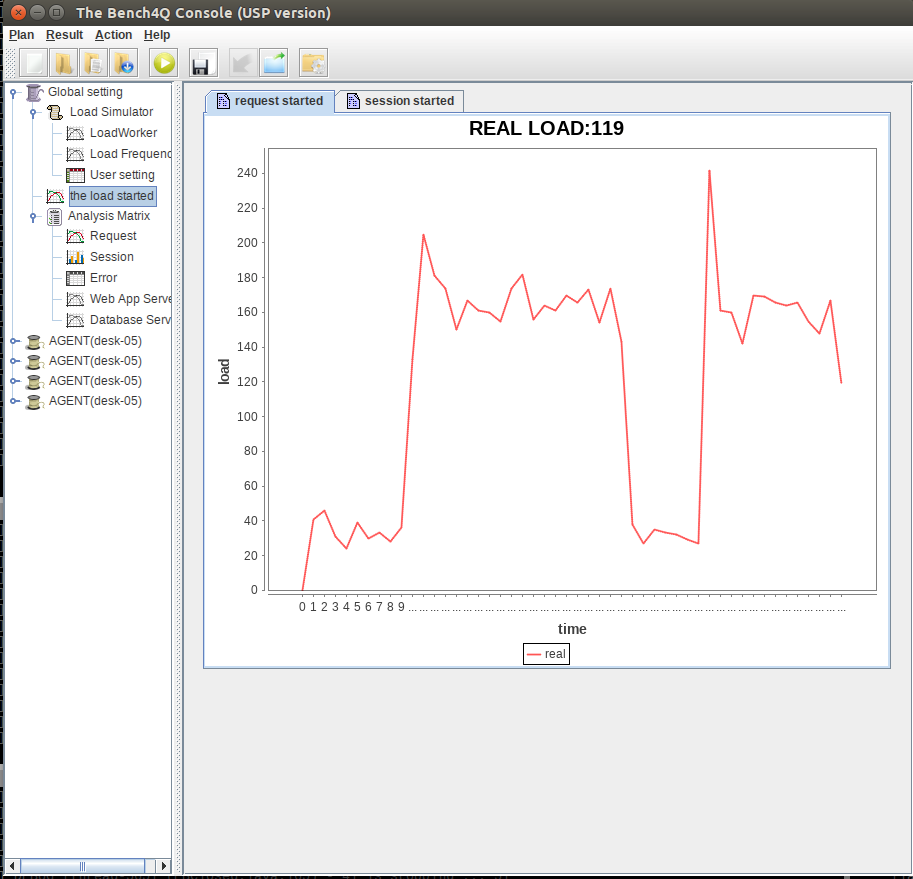
\includegraphics[scale=0.25]{../monograph/images/grafico-carga-modulada-teste.png}
			\label{fig:grafico-carga-modulada-teste}
		\end{subfigure}
		\label{fig:carga-modulada-teste}
	\end{figure}
\end{frame}

